\chapter{Symmetric instability in a cross-equatorial deep western boundary current}
\begin{quote}
    \textit{Brrrrrrr} --- Fraser Goldsworth
\end{quote}

\section{Introduction}
Density staircases are step like features which can be seen in plots of seawater density against depth, and they are ubiquitous in the global ocean~\cite{Stern1960,Schmitt1987,Melling1984,Tait1968,Johannessen1974,Lambert1977},. The staircases consist of alternating well mixed regions with low stratification, and thin interfaces with high stratification. The high stratification interfaces can form ``mixing barriers'' which inhibit the vertical transport of water properties such as heat and salt, whereas mixing is enhanced in the well mixed regions. This can affect both diapycnal mixing and water mass transformation rates ~\cite{Schmitt2005}. Many staircases form as a result of double diffusion convection, a mechanism which requires certain conditions regarding the saline stratification relative to the thermal stratification to be met~\cite{Merryfield2000}. Other staircase generation mechanisms exist, for example inhomogeneous mixing~\cite{Balmforth1998}.
% Come back to the last two sentences above.

The Atlantic meridional overturning circulation (AMOC) is a global scale circulation that is important in transporting heat and salt both laterally and vertically, including between hemispheres~\cite{Jackson2015}. There are two important cross-equatorial components to the AMOC --- the northward flowing, surface intensified North Brazil Current, and the southward flowing deep western boundary current~\cite{Bower2019}. At $5^\circ$S the deep western boundary current transports $25.5 \pm 8.3$~Sv, sits between 1,200~m and 3,600~m below the surface, with a width of approximately 100~km and a peak velocity of around 20~cm$\,$s$^{-1}$~\cite{Schott2005}. \citet{Goldsworth2021} show that cross-equatorial western boundary currents such as this may be susceptible to symmetric instability.

Symmetric instability is a type of sub-mesoscale instability which occurs when the Ertel potential vorticity of a flow has the opposite sign to the planetary vorticity~\cite{Stone1966, Hoskins1974}.  Potential vorticity is defined as
\begin{equation}
    Q = (\mathbf{f} + \mathbf{\nabla} \times \mathbf{u}) \cdot \mathbf{\nabla}b \, ,
\end{equation}
where $\mathbf{f}$ is the planetary vorticity vector, $\mathbf{u}$ is the velocity field of the flow $b = - g \rho / \rho_0$ is the buoyancy field. Potential vorticity with sign opposite to that of the (vertical component of) planetary vorticity is often described as anomalous. Symmetric instability may be excited in cross-equatorial flows as potential vorticity is materially conserved, whereas at the equator planetary vorticity changes sign. This means fluid originating from the northern hemisphere which has positive potential vorticity (in order for the flow to be stable to symmetric instability) may become symmetrically unstable upon crossing the equator, as planetary vorticity is negative in the southern hemisphere~\cite{Goldsworth2021}. The excitement of symmetric instability creates stacked overturning cells in the plane perpendicular to the flow. These overturning cells act to set the potential vorticity of the flow to zero. Potential vorticity of zero is often described as being marginal.

Anomalous potential vorticity can be generated in one of two ways, either by changing the sign of the potential vorticity or by changing the sign of the planetary vorticity. As potential vorticity is materially conserved, a fluid may only change the sign of its potential vorticity via frictional momentum forcing or diabatic buoyancy forcing. These processes typically alter only the local potential vorticity and occur in boundary layers, meaning symmetric instability tends to be confined to either the surface boundary layer or the sloping bottom boundary layer. A change in sign of planetary vorticity, however, generates anomalous potential vorticity throughout the water column. This makes cross-equatorial symmetric instability distinct from instabilities generated by potential vorticity forcing. A host of recent studies have identified regions were cross-equatorial symmetric instability may be excited~\cite{Goldsworth2021, Forryan2021,Zhou2022,Jakoboski2019}. In this paper we will investigate the excitement of symmetric instability in a cross-equatorial deep western boundary current, away from the surface and frictional bottom boundary layers.

In section~\ref{sec:methods} an idealised numerical model of a deep western boundary current crossing the equator is described. In section~\ref{sec:randd} we show that the model output shows signs of density staircases and the excitement of symmetric instability, and propose that the staircases are generated as a result of the symmetric instability's excitement. Finally, in section~\ref{sec:conc} we summarise our findings and outline our plans for future work.

\section{Methods}
\label{sec:methods}
Simulations of an idealised Deep Western Boundary Current crossing the equator were performed using the MITgcm, checkpoint 68i, on the ARCHER2 HPC facility. The domain size is 600 km in the zonal, 3,600 km in the meridional and 4,500 m in the vertical. The horizontal grid spacing is 1 km and the vertical grid spacing 10 m. The time-step is 144 s and the model is integrated for a total of 239 days. The model domain is sited on a $\beta$-plane, with the equator placed 2,000 km north of the southern boundary. $\beta$ is set to $2.3 \times 10^{-11}$ s$^{-1}\,$m$^{-1}$, and the non-traditional Coriolis parameter to $1.5 \times 10^{-4}$ s$^{-1}$.

At the surface a rigid lid boundary condition is employed. The lateral boundary condition is set to be free-slip and the bottom boundary condition to no-slip. The model has sloping bathymetry which can be seen in figure~\ref{fig:fig1}b. The model is initialised by setting the meridional velocity and density profile to those shown in figure~\ref{fig:fig1}b, and with a zonal velocity of zero. The model is forced by prescribing the meridional velocity, zonal velocity, and the density, at the northern and southern domain boundaries. The same fields used to initialise the model are used as boundary conditions. A sponge is placed at the northern and southern edges of the domain. The northern sponge is 100 km thick and the southern sponge 300 km thick. The inverse relaxation time-scale varies from $1\times 10^{-5}$ s$^{-1}$ (corresponding to a time scale of around 1.2 days) at the outer boundaries to 0 at the inner. The inverse relaxation time-scale has a $\tanh$ shape, with a characteristic length-scale of 5 km in the northern sponge and 10 km in the southern.

A linear equation of state is used, with a reference density of 1022.73 kg\,m$^{-3}$ and thermal expansion coefficient of $2 \times 10^{-4}$ K$^{-1}$. The thermal diffusion coefficient is set to $1 \times 10^{-5}$ m$^{2}$\,s$^{-1}$. A second order-moment Prather with flux limiter advection scheme was used. Salinity was set to zero throughout the model.

Momentum dissipation is provided by a vertical Laplacian viscosity of $4 \times 10^{-4}$ m$^{2}$\,s$^{-1}$ and an adaptive biharmonic Smagorinsky viscosity.

Model configuration files and processed outputs are available from~\citet{code} and~\citet{data}. The subsequent analysis made heavy use of the open source xarray~\cite{xarray} and Dask~\cite{Dask} software libraries. Potential vorticity was calculated using the algorithm of~\citet{Morel2019}.

\begin{figure}[h]
    \centering
    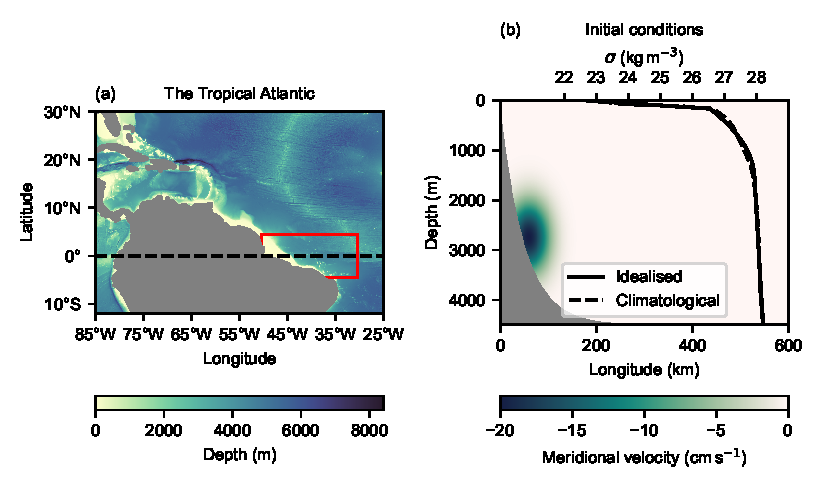
\includegraphics[width=\textwidth]{../figures/Figure1.pdf}
    \caption{(a) A map of the tropical Atlantic and its bathymetry. Climatological profiles of neutral density were aggregated from the area enclosed by the red rectangle. Bathymetry data from~\citet{GEBCO2020}. (b) Initial meridional velocity profile and density profile (solid line) used as initial conditions and boundary conditions for the model. The velocity profile is based on observations by~\citet{Schott2005}, and the density profile on the climatological mean (dashed line)~\citep{WOA2018}.}
    \label{fig:fig1}
\end{figure}

\section{Results \& discussion}
\label{sec:randd}
Figure~\ref{fig:staircase}b shows the squared buoyancy frequency in the model after 239 days of integration at 250 km south. Immediately apparent are the thin, sharp regions of high stratification (so called ``mixing barriers'') separating larger regions of well mixed waters with low and uniform stratification. Moving to 500 km south, we see in figure~\ref{fig:staircase}c that some of the weaker barriers have dissipated, however the stronger barriers remain. Figure~\ref{fig:staircase}a shows the squared buoyancy frequency at the equator. Towards the right of the current's core we  see some weak mixing barriers.

Figure~\ref{fig:StaircaseMechanism}a shows the average of the meridional component of relative vorticity 250 km south of the equator between 234 and 239  days of model integration. This can be thought of as a crude proxy for a zonal overturning streamfunction. We consider it here as the true zonal overturning streamfunction is ill-defined, since the flow is not invariant in the meridional direction. Looking at the vorticity as akin to a streamfunction, we see that there are a series of counter-rotating stacked overturning cells between around 1,750 m and 3,500 m below the surface. Comparing with figure~\ref{fig:staircase}b we see that the structure of the buoyancy frequency squared and the meridional vorticity are remarkably similar, with the horizontal edges of the overturning cells (vorticity zeros) approximately coinciding with the locations of the mixing barriers. This is shown more clearly in figure~\ref{fig:StaircaseMechanism}b. The black line shows $\sigma$  plotted as a function of  depth at 250 km south and 90 km west (the location of the magenta lines and points shown in the other  figures). The grey line shows the meridional component of relative vorticity at the same point. Both quantities  have  been averaged over the time period spanning 234 to 239 days. The treads of the steps in $\sigma$ correspond to mixing barriers and the risers to well mixed regions. When comparing $\sigma$ and the meridional vorticity we again see that the mixing barriers tend to coincide with vorticity zeros, whereas the mixing barriers coincide with vorticity extrema. This suggest that the inhomegeneous mixing driven by the overturning cells is what is causing the formation of the staircases.

\begin{figure}[h]
    \centering
    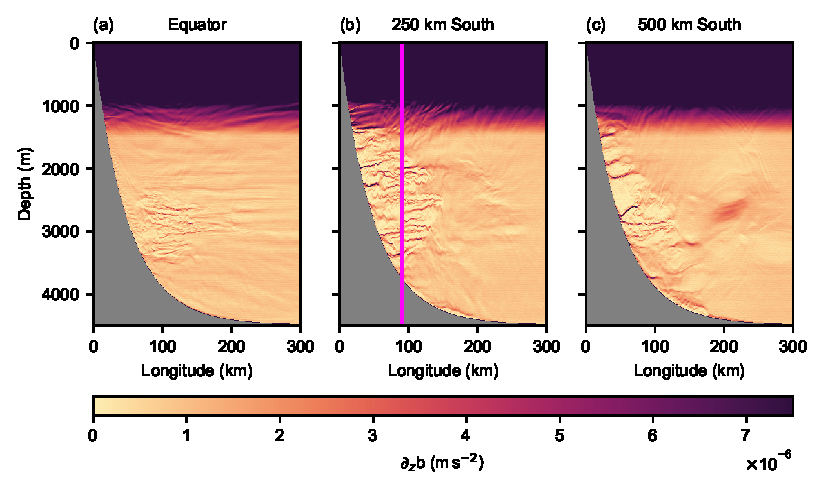
\includegraphics{../figures/Figure2.pdf}
    \caption{Squared buoyancy frequency after 239 days of model integration plotted at (a) 250 km south of the equator,  (b) 500 km south of the equator and (c) 600 km south of the equator. The figures show the presence of mixing barriers (thin filaments of strong stratification) separated by well mixed regions of low stratification. The magenta line indicates the location of the vorticity and density profiles shown in figure~\ref{fig:StaircaseMechanism}.}
    \label{fig:staircase}
\end{figure}

We believe that the overturning cells are generated by symmetric instability and that it is this overturning that goes on to generate the density staircases, as opposed to the density staircases somehow inducing overturning. Previous work by \citet{Goldsworth2021} has demonstrated that western boundary currents can become unstable when crossing the equator as they advect anomalous potential vorticity from one hemisphere into the other. In figure~\ref{fig:PV}a, which shows the potential vorticity on the $\sigma$ = 28.04 surface, we can see the advection of positive potential vorticity from the northern hemisphere into the southern hemisphere, meaning we may expect to see symmetric instability excited south of the equator. The excitement of the instability is apparent in a region from around 25 km to 600 km south of the equator. Figures~\ref{fig:PV}b, c, and d show the potential vorticity as a function of depth and longitude at, the equator, 250 km south and 500 km south respectively, after 239 days of model integration. At the equator we see the advection of waters with anomalous potential vorticity into the southern hemisphere. At 250 km south we can see the excitement of symmetric instability, and by 500 km south we can see large pools of neutral potential vorticity suggesting the waters here have experienced symmetric instability, with the excitement of symmetric instability still underway at around 3,000 m of depth. In figure~\ref{fig:PV}b we also see symmetric instability like patterns in a region of negative potential vorticity. This suggests these waters with negative potential vorticity were undergoing symmetric instability in the northern hemisphere  before being advected south of the equator. This also explains the presence of the weak staircases at the equator seen in figure~\ref{fig:staircase}a.

Unlike in the study of~\cite{Goldsworth2021}, we see the excitement of symmetric instability close to the equator followed by the formation of eddies, whereas in the former study we see the spinning up of large anti-cyclonic eddies followed by the excitement of symmetric instability further away from the equator. This is due to the reduced growth rate of barotropic instability in the deep western boundary current, meaning that symmetric instability dominates over short time-scales. This is further exacerbated by the anti-cyclonic eddies seen by~\cite{Goldsworth2021}, which act to reduce the growth rate of the symmetric instability in their experiments, allowing anomalous potential vorticity to persist whilst the eddies grow~\cite{Buckingham2021}. 

\begin{figure}
    \centering
    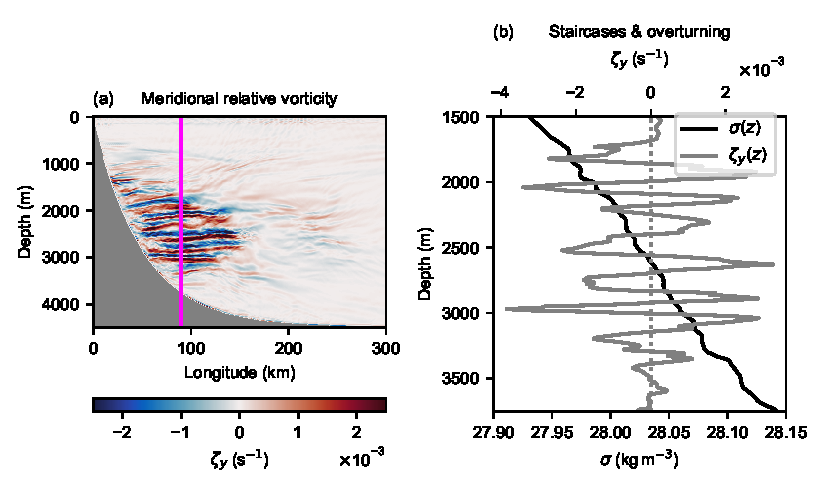
\includegraphics{../figures/Figure3.pdf}
    \caption{(a) Time mean meridional component of relative vorticity between 234 and 239 days of model integration, plotted as a function of longitude and depth. Alternating red and blue cells indicate the presence of stacked zonal overturning cells. (b) Density (black line) and time mean meridional component of relative vorticity (grey line) plotted as a function of depth at 90 km west and 250 km south (shown on other figures as a magenta line and point). Vorticity extrema coincide with well mixed regions and zeros with mixing barriers suggesting the density staircases are formed by the overturning cells.}
    \label{fig:StaircaseMechanism}
\end{figure}

\begin{figure}[hp]
    \centering
    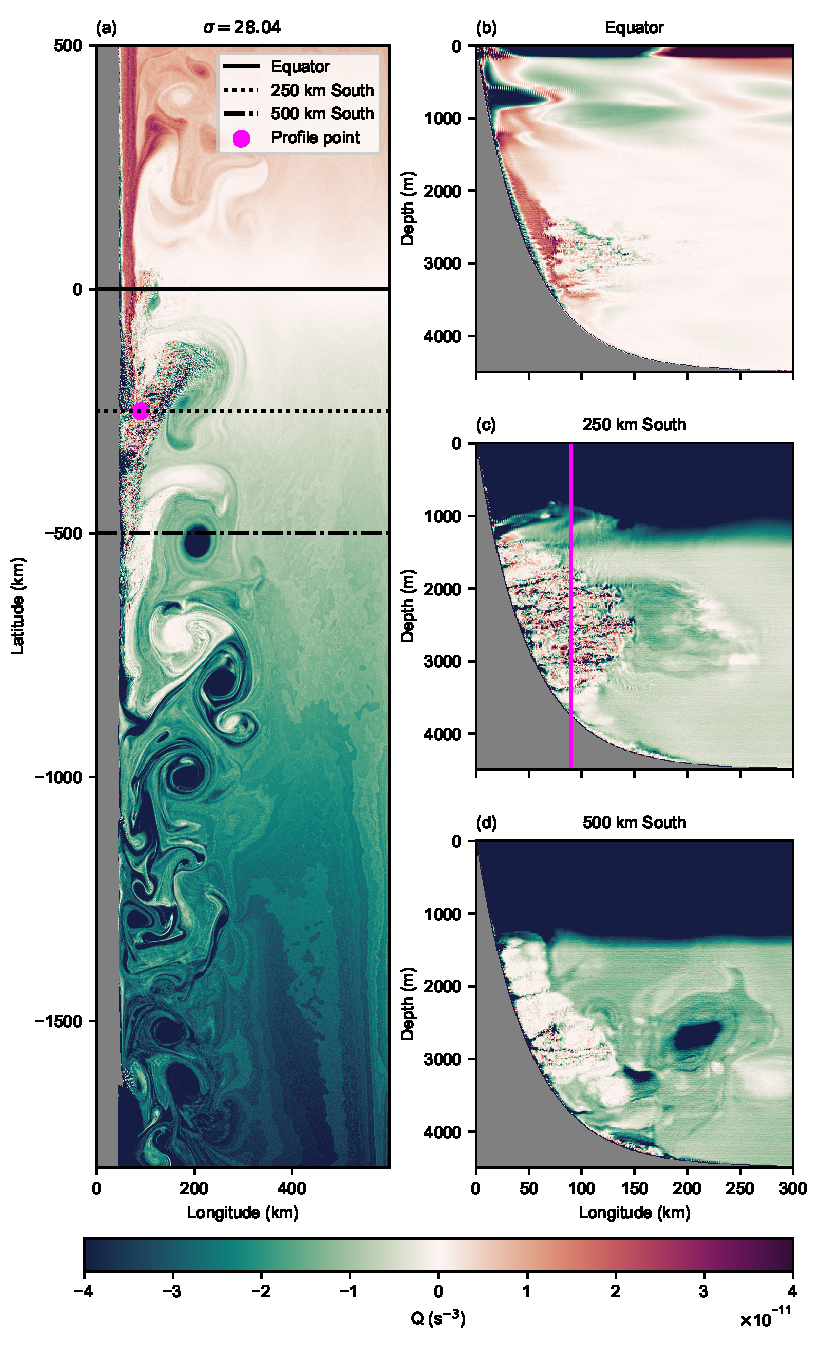
\includegraphics{../figures/Figure4.pdf}
    \caption{Potential vorticity after 239 days of model integration plotted on (a) the $\sigma = 28.04$ surface, (b) at the equator, (c) at 250 km south of the equator, and (d) at 500 km south of the equator. Black lines show the latitudes at which sections have been plotted. The figures show the advection of anomalous potential vorticity from the northern hemisphere into the southern hemisphere and the excitement of symmetric instability underway. The magenta line and point indicate the location of the vorticity and density profiles shown in figure~\ref{fig:StaircaseMechanism}.}
    \label{fig:PV}
\end{figure}

\section{A simplified model of staircse formation}

\begin{equation}
    \pdv{b}{t} = - u \pdv{b}{x} - w \pdv{b}{z} + \kappa \pdv[2]{b}{z}
\end{equation}

\section{Conclusions}
\label{sec:conc}
Density staircases are step like features which become apparent when density is plotted as a function of depth and are common throughout the Earth's oceans. In an idealised model of a deep western boundary current crossing the equator we see density staircases form. The staircases are generated by overturning cells which are in turn generated by the excitement of symmetric instability as the current crosses the equator. Symmetric instability in cross-equatorial flows is excited due to the advection of anomalous potential vorticity from one hemisphere to another. The stacked overturning cells that generate the staircases are, however, a feature of symmetric instability regardless of what is forcing its excitement, suggesting we may see staircase formation in other symmetrically unstable flows --- including when anomalous potential vorticity is induced by frictional torques or diabatic processes.

It is thought that diapycnal mixing may play an important role in closing the overturning budget of the Atlantic Meridional Overturning Circulation's deep limb. The amount of diapycnal mixing induced by symmetric instability in the deep western boundary current should be investigated further to ascertain whether the process may help to close the overturning budget.